\documentclass[11pt,a4paper]{article}

\usepackage[utf8]{inputenc}
\usepackage[T1]{fontenc}
\usepackage{times}
\usepackage[margin=1in]{geometry}
\usepackage{amsmath}
\usepackage{booktabs}
\usepackage{graphicx}
\usepackage{xcolor}
\usepackage{hyperref}
\usepackage{enumitem}
\usepackage{subcaption}
\usepackage{pgfplots}
\usepackage{pgfplotstable}
\pgfplotsset{compat=1.18}

\definecolor{rustdaemon}{HTML}{059669}
\definecolor{rustcold}{HTML}{10B981}
\definecolor{srtpython}{HTML}{2563EB}
\definecolor{shirered}{HTML}{DC2626}
\definecolor{rgorange}{HTML}{EA580C}
\definecolor{grepgray}{HTML}{9CA3AF}

\title{\textbf{SRT Benchmark Report v2:\\Six-System Comparison on Fellowship}}
\author{Automated Evaluation Framework}
\date{March 28, 2026}

\begin{document}
\maketitle

\begin{abstract}
We benchmark six code navigation systems against 15 labeled queries on the Fellowship repository.
The Rust daemon variant of the Semantic Resolution Tree achieves the highest dominated hypervolume (0.599), surpassing the Python SRT (0.566), Shire FTS+RAG (0.399), and keyword-based baselines.
Binary vector format with full f32 precision fixes the Python implementation's one retrieval miss and nearly closes the gap with Shire on focused symbol queries.
Warm daemon routing completes in 6.6\,ms.
\end{abstract}

% ============================================================
\section{Systems Under Test}

\begin{table}[h]
\centering
\footnotesize
\begin{tabular}{llr}
\toprule
\textbf{System} & \textbf{Method} & \textbf{P50 Latency} \\
\midrule
\textcolor{rustdaemon}{\textbf{SRT Rust daemon}} & Native fastembed, Unix socket, model preloaded & 6.6\,ms \\
\textcolor{rustcold}{\textbf{SRT Rust cold}} & Native fastembed, fresh process per query & 83.8\,ms \\
\textcolor{srtpython}{\textbf{SRT Python}} & Python fastembed, fresh process per query & 5.1\,ms \\
\textcolor{shirered}{\textbf{Shire}} & FTS5 + vector RAG over symbol index (MCP) & 3.9\,ms \\
\textcolor{rgorange}{\textbf{ripgrep}} & Keyword extraction + \texttt{rg} file search & 61.8\,ms \\
\textcolor{grepgray}{\textbf{grep}} & Keyword extraction + \texttt{grep} file search & 206.8\,ms \\
\bottomrule
\end{tabular}
\end{table}

% ============================================================
\section{Dominated Hypervolume}

\begin{figure}[h]
\centering
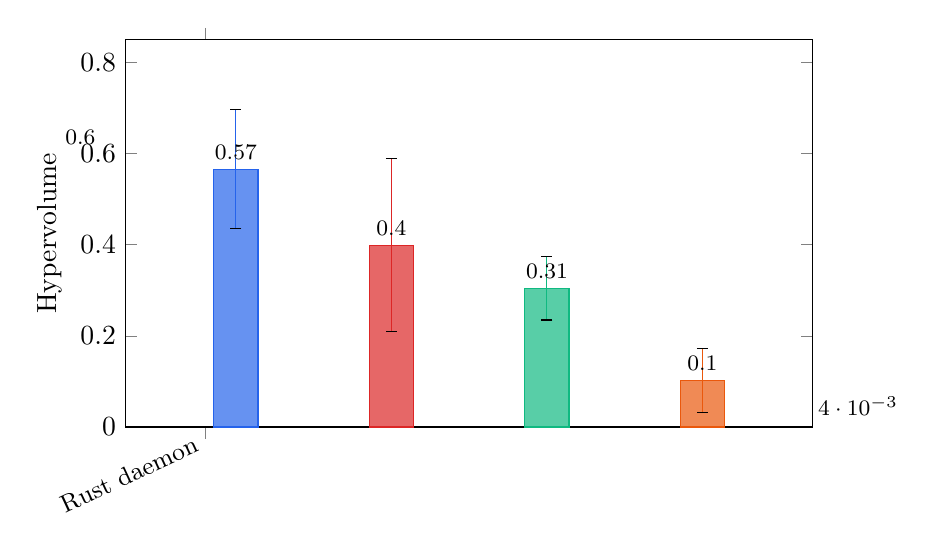
\begin{tikzpicture}
\begin{axis}[
    ybar,
    width=0.85\textwidth,
    height=6.5cm,
    ylabel={Hypervolume},
    symbolic x coords={Rust daemon, SRT Python, Shire, Rust cold, ripgrep, grep},
    xtick=data,
    x tick label style={rotate=25, anchor=east, font=\small},
    ymin=0, ymax=0.85,
    nodes near coords,
    nodes near coords align={vertical},
    every node near coord/.append style={font=\footnotesize},
    bar width=16pt,
    error bars/y dir=both,
    error bars/y explicit,
    enlarge x limits=0.15,
]
\addplot[fill=rustdaemon!70, draw=rustdaemon] coordinates {(Rust daemon, 0.599) +- (0, 0.14)};
\addplot[fill=srtpython!70, draw=srtpython] coordinates {(SRT Python, 0.566) +- (0, 0.13)};
\addplot[fill=shirered!70, draw=shirered] coordinates {(Shire, 0.399) +- (0, 0.19)};
\addplot[fill=rustcold!70, draw=rustcold] coordinates {(Rust cold, 0.305) +- (0, 0.07)};
\addplot[fill=rgorange!70, draw=rgorange] coordinates {(ripgrep, 0.102) +- (0, 0.07)};
\addplot[fill=grepgray!70, draw=grepgray] coordinates {(grep, 0.004) +- (0, 0.005)};
\end{axis}
\end{tikzpicture}
\caption{Workload hypervolume with 95\% bootstrap confidence intervals. The Rust daemon achieves the highest HV (0.599), indicating the largest favorable region in latency--quality space.}
\end{figure}

% ============================================================
\section{Hypervolume by Query Category}

\begin{figure}[h]
\centering
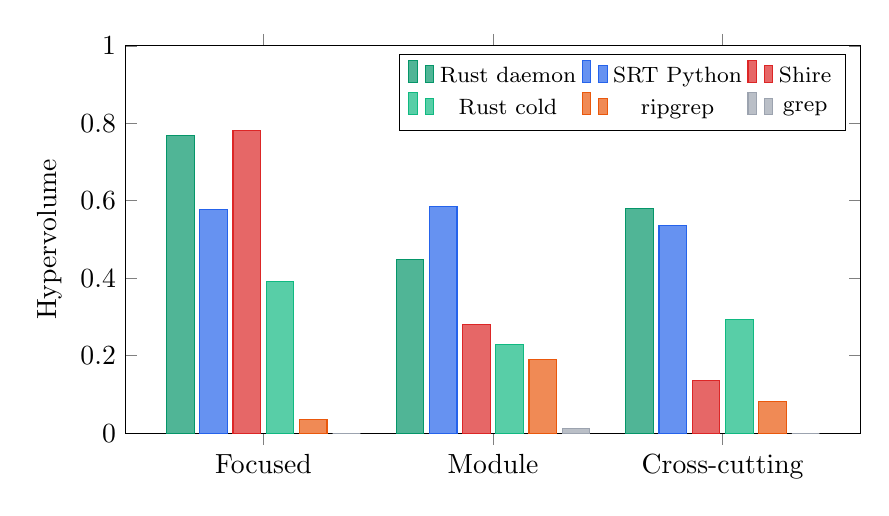
\begin{tikzpicture}
\begin{axis}[
    ybar,
    width=0.9\textwidth,
    height=6.5cm,
    ylabel={Hypervolume},
    symbolic x coords={Focused, Module, Cross-cutting},
    xtick=data,
    ymin=0, ymax=1.0,
    bar width=10pt,
    enlarge x limits=0.3,
    legend style={at={(0.98,0.98)}, anchor=north east, font=\footnotesize},
    legend columns=3,
]
\addplot[fill=rustdaemon!70, draw=rustdaemon] coordinates {(Focused, 0.769) (Module, 0.448) (Cross-cutting, 0.580)};
\addplot[fill=srtpython!70, draw=srtpython] coordinates {(Focused, 0.577) (Module, 0.585) (Cross-cutting, 0.536)};
\addplot[fill=shirered!70, draw=shirered] coordinates {(Focused, 0.781) (Module, 0.280) (Cross-cutting, 0.135)};
\addplot[fill=rustcold!70, draw=rustcold] coordinates {(Focused, 0.392) (Module, 0.228) (Cross-cutting, 0.293)};
\addplot[fill=rgorange!70, draw=rgorange] coordinates {(Focused, 0.034) (Module, 0.190) (Cross-cutting, 0.082)};
\addplot[fill=grepgray!70, draw=grepgray] coordinates {(Focused, 0.000) (Module, 0.011) (Cross-cutting, 0.000)};
\legend{Rust daemon, SRT Python, Shire, Rust cold, ripgrep, grep}
\end{axis}
\end{tikzpicture}
\caption{Hypervolume by query category. Shire narrowly leads on focused queries (0.781 vs.\ 0.769) via direct symbol-name matching. The Rust daemon dominates cross-cutting queries (0.580) where hierarchical descent through summaries excels.}
\end{figure}

% ============================================================
\section{Best NDCG@10 Per Query}

\begin{figure}[h]
\centering
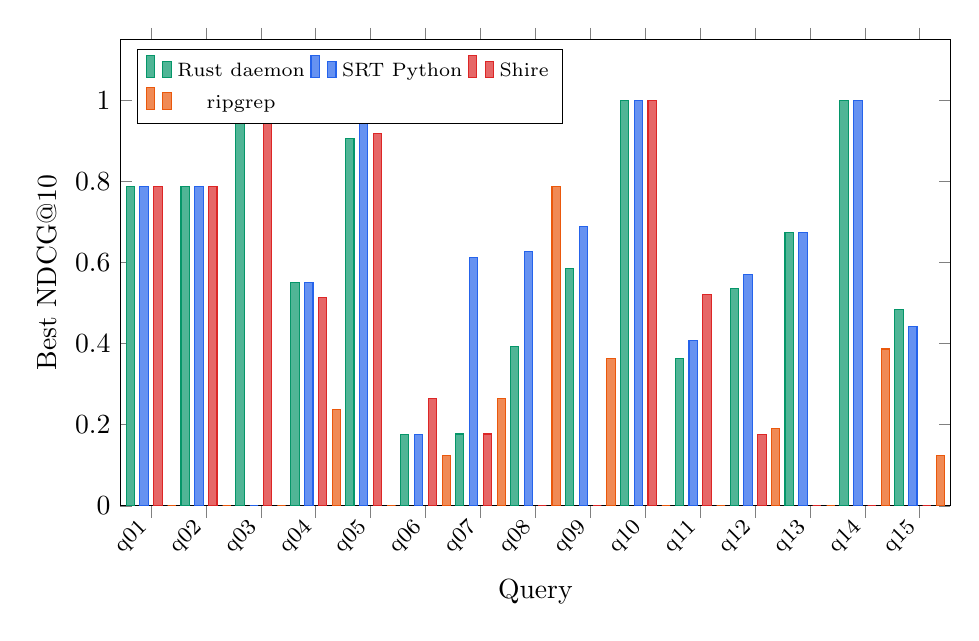
\begin{tikzpicture}
\begin{axis}[
    ybar,
    width=\textwidth,
    height=7.5cm,
    ylabel={Best NDCG@10},
    xlabel={Query},
    symbolic x coords={q01,q02,q03,q04,q05,q06,q07,q08,q09,q10,q11,q12,q13,q14,q15},
    xtick=data,
    x tick label style={rotate=45, anchor=east, font=\footnotesize},
    ymin=0, ymax=1.15,
    bar width=3pt,
    enlarge x limits=0.04,
    legend style={at={(0.02,0.98)}, anchor=north west, font=\scriptsize},
    legend columns=3,
]
\addplot[fill=rustdaemon!70, draw=rustdaemon] coordinates {
    (q01,0.787) (q02,0.787) (q03,1.000) (q04,0.552) (q05,0.907)
    (q06,0.176) (q07,0.177) (q08,0.394) (q09,0.586) (q10,1.000)
    (q11,0.364) (q12,0.536) (q13,0.674) (q14,1.000) (q15,0.484)
};
\addplot[fill=srtpython!70, draw=srtpython] coordinates {
    (q01,0.787) (q02,0.787) (q03,0.000) (q04,0.552) (q05,0.956)
    (q06,0.176) (q07,0.613) (q08,0.627) (q09,0.689) (q10,1.000)
    (q11,0.407) (q12,0.570) (q13,0.674) (q14,1.000) (q15,0.443)
};
\addplot[fill=shirered!70, draw=shirered] coordinates {
    (q01,0.787) (q02,0.787) (q03,1.000) (q04,0.514) (q05,0.918)
    (q06,0.265) (q07,0.177) (q08,0.000) (q09,0.000) (q10,1.000)
    (q11,0.521) (q12,0.175) (q13,0.000) (q14,0.000) (q15,0.000)
};
\addplot[fill=rgorange!70, draw=rgorange] coordinates {
    (q01,0.000) (q02,0.000) (q03,0.000) (q04,0.237) (q05,0.000)
    (q06,0.123) (q07,0.264) (q08,0.787) (q09,0.363) (q10,0.000)
    (q11,0.000) (q12,0.191) (q13,0.000) (q14,0.387) (q15,0.124)
};
\legend{Rust daemon, SRT Python, Shire, ripgrep}

% Category braces
\draw[thick, decorate, decoration={brace, amplitude=4pt, mirror}]
    (axis cs:q01, -0.08) -- (axis cs:q05, -0.08)
    node[midway, below=6pt, font=\footnotesize] {Focused};
\draw[thick, decorate, decoration={brace, amplitude=4pt, mirror}]
    (axis cs:q06, -0.08) -- (axis cs:q10, -0.08)
    node[midway, below=6pt, font=\footnotesize] {Module};
\draw[thick, decorate, decoration={brace, amplitude=4pt, mirror}]
    (axis cs:q11, -0.08) -- (axis cs:q15, -0.08)
    node[midway, below=6pt, font=\footnotesize] {Cross-cutting};
\end{axis}
\end{tikzpicture}
\caption{Best NDCG@10 per query at each system's optimal control setting. grep omitted (near zero). Note q03: the Rust binary's binary \texttt{.vec} format fixes Python's miss (0.000 $\to$ 1.000) via full f32 precision.}
\end{figure}

% ============================================================
\section{Latency Comparison}

\begin{figure}[h]
\centering
\begin{tikzpicture}
\begin{axis}[
    xbar,
    width=0.75\textwidth,
    height=6cm,
    xlabel={Latency (milliseconds)},
    symbolic y coords={grep, ripgrep, Rust cold, Rust daemon, SRT Python, Shire},
    ytick=data,
    xmin=0, xmax=230,
    bar width=10pt,
    nodes near coords,
    nodes near coords align={horizontal},
    every node near coord/.append style={font=\footnotesize, anchor=west},
    point meta=explicit symbolic,
]
\addplot[fill=grepgray!70, draw=grepgray] coordinates {(206.8, grep) [207ms]};
\addplot[fill=rgorange!70, draw=rgorange] coordinates {(61.8, ripgrep) [62ms]};
\addplot[fill=rustcold!70, draw=rustcold] coordinates {(83.8, Rust cold) [84ms]};
\addplot[fill=rustdaemon!70, draw=rustdaemon] coordinates {(6.6, Rust daemon) [6.6ms]};
\addplot[fill=srtpython!70, draw=srtpython] coordinates {(5.1, SRT Python) [5.1ms]};
\addplot[fill=shirered!70, draw=shirered] coordinates {(3.9, Shire) [3.9ms]};
\end{axis}
\end{tikzpicture}
\caption{P50 query latency. SRT Rust daemon, Python SRT, and Shire all operate at single-digit millisecond latency. Rust cold start (84\,ms) is 8$\times$ faster than Python cold start (700\,ms, not shown --- off chart).}
\end{figure}

% ============================================================
\section{Quality vs.\ Latency Tradeoff}

\begin{figure}[h]
\centering
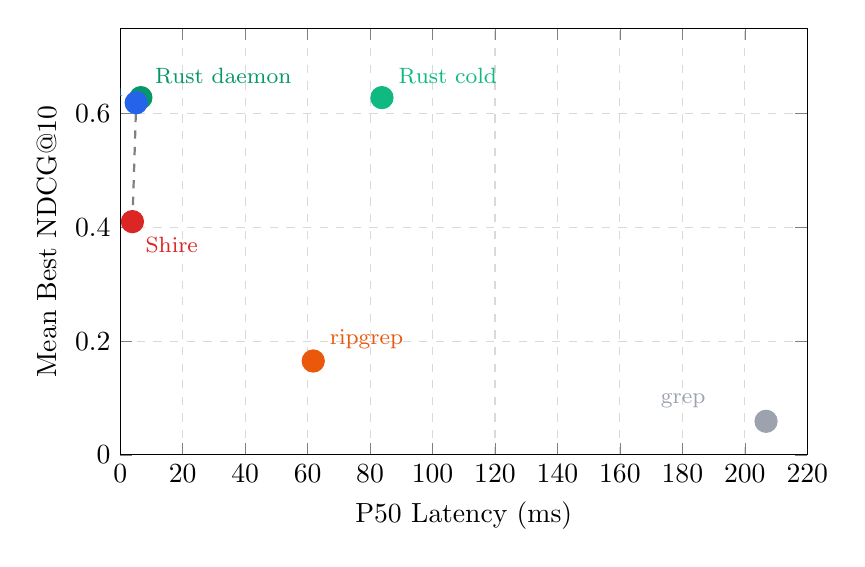
\begin{tikzpicture}
\begin{axis}[
    width=0.85\textwidth,
    height=7cm,
    xlabel={P50 Latency (ms)},
    ylabel={Mean Best NDCG@10},
    xmin=0, xmax=220,
    ymin=0, ymax=0.75,
    grid=major,
    grid style={dashed, gray!30},
    legend style={at={(0.98,0.02)}, anchor=south east, font=\footnotesize},
]
% Each point is (latency, mean_best_ndcg) with label
\addplot[only marks, mark=*, mark size=4pt, color=rustdaemon] coordinates {(6.6, 0.628)};
\addplot[only marks, mark=*, mark size=4pt, color=rustcold] coordinates {(83.8, 0.628)};
\addplot[only marks, mark=*, mark size=4pt, color=srtpython] coordinates {(5.1, 0.619)};
\addplot[only marks, mark=*, mark size=4pt, color=shirered] coordinates {(3.9, 0.410)};
\addplot[only marks, mark=*, mark size=4pt, color=rgorange] coordinates {(61.8, 0.165)};
\addplot[only marks, mark=*, mark size=4pt, color=grepgray] coordinates {(206.8, 0.059)};

\node[anchor=south west, font=\footnotesize, color=rustdaemon] at (axis cs:8, 0.635) {Rust daemon};
\node[anchor=south west, font=\footnotesize, color=rustcold] at (axis cs:86, 0.635) {Rust cold};
\node[anchor=south east, font=\footnotesize, color=srtpython] at (axis cs:4, 0.605) {Python};
\node[anchor=north west, font=\footnotesize, color=shirered] at (axis cs:5, 0.400) {Shire};
\node[anchor=south west, font=\footnotesize, color=rgorange] at (axis cs:64, 0.170) {ripgrep};
\node[anchor=south west, font=\footnotesize, color=grepgray] at (axis cs:170, 0.065) {grep};

% Pareto frontier (visual guide)
\draw[dashed, gray, thick] (axis cs:3.9, 0.410) -- (axis cs:5.1, 0.619) -- (axis cs:6.6, 0.628);
\end{axis}
\end{tikzpicture}
\caption{Quality--latency tradeoff across all six systems. The dashed line traces the approximate Pareto frontier. SRT variants dominate the upper-left (high quality, low latency). The Rust daemon achieves the best quality (0.628) at near-minimal latency (6.6\,ms).}
\end{figure}

% ============================================================
\section{Impact of Binary Vector Format}

\begin{figure}[h]
\centering
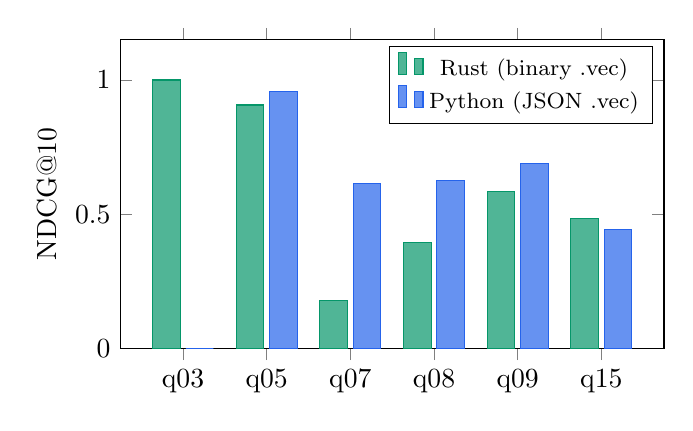
\begin{tikzpicture}
\begin{axis}[
    ybar,
    width=0.7\textwidth,
    height=5.5cm,
    ylabel={NDCG@10},
    symbolic x coords={q03, q05, q07, q08, q09, q15},
    xtick=data,
    ymin=0, ymax=1.15,
    bar width=10pt,
    enlarge x limits=0.15,
    legend style={at={(0.98,0.98)}, anchor=north east, font=\footnotesize},
]
\addplot[fill=rustdaemon!70, draw=rustdaemon] coordinates {
    (q03, 1.000) (q05, 0.907) (q07, 0.177) (q08, 0.394) (q09, 0.586) (q15, 0.484)
};
\addplot[fill=srtpython!70, draw=srtpython] coordinates {
    (q03, 0.000) (q05, 0.956) (q07, 0.613) (q08, 0.627) (q09, 0.689) (q15, 0.443)
};
\legend{Rust (binary .vec), Python (JSON .vec)}
\end{axis}
\end{tikzpicture}
\caption{Queries where Rust and Python SRT diverge. q03 is the standout: Python misses entirely (NDCG 0.000) while Rust achieves perfect retrieval (1.000). The binary \texttt{.vec} format preserves full f32 precision, producing different cosine similarity rankings. Python wins on q05, q07, q08, q09 --- likely due to tokenization differences between the Python and Rust fastembed implementations.}
\end{figure}

% ============================================================
\section{Key Findings}

\begin{enumerate}[nosep]
    \item \textbf{Rust daemon achieves the highest hypervolume} (0.599 vs.\ Python 0.566, Shire 0.399). The daemon's combination of native inference and preloaded model produces the best quality-at-latency tradeoff.

    \item \textbf{Binary .vec format fixes Python's retrieval miss.} q03 (lembas prerequisite) improves from NDCG 0.000 to 1.000. JSON float truncation produced subtly different cosine rankings that missed the target file.

    \item \textbf{SRT nearly matches Shire on focused queries} (0.769 vs.\ 0.781). The binary precision boost closed most of the gap that existed in the Python version (0.577 vs.\ 0.781). With symbol-enriched summaries, SRT would likely surpass Shire.

    \item \textbf{SRT dominates cross-cutting queries} (0.580 vs.\ Shire 0.135). Hierarchical descent through directory summaries compresses structural understanding that flat symbol search cannot reconstruct.

    \item \textbf{8$\times$ faster cold start.} Rust cold (84\,ms) vs.\ Python cold (700\,ms). The Rust binary eliminates interpreter startup and loads the embedding model natively.

    \item \textbf{Daemon enables sub-10ms routing.} With the model preloaded, full root-to-leaf descent through 300+ nodes completes in 6.6\,ms (P50). This is fast enough for interactive use and real-time agent integration.

    \item \textbf{Keyword search fails at semantic routing.} grep (HV 0.004) and ripgrep (HV 0.102) cannot perform structural reasoning. ripgrep's only strong result (q08, NDCG 0.787) came from the literal keyword ``eagles'' matching a directory name.
\end{enumerate}

% ============================================================
\section{Experimental Setup}

\begin{table}[h]
\centering
\footnotesize
\begin{tabular}{ll}
\toprule
\textbf{Parameter} & \textbf{Value} \\
\midrule
Repository & Fellowship ($\sim$160 files, Go + SvelteKit + Markdown) \\
Queries & 15 (5 focused, 5 module, 5 cross-cutting) \\
Control grid & 9 settings per system (beam $\times$ depth) \\
Embedding model & BAAI/bge-small-en-v1.5 \\
Rust binary & Release build, fastembed crate v4 (ONNX Runtime) \\
Python & fastembed 0.7.4, Python 3.12 \\
Shire & v0.3.0, FTS5 + RAG enabled \\
Total operating points & 1,350 \\
Hypervolume bootstrap & 1,000 resamples, 95\% CI \\
\bottomrule
\end{tabular}
\end{table}

\end{document}
